\chapter{Chapter title}\index{chapter}
The chapter usually opens with a small section at full width. This section has the purpose to introduce the content of the chapter.

\lipsum[1]
\stdsection{Physics and other sciences}
A standard section\index{section!standard} is rendered with blue background. It is numbered and the text spans over part of the full width, leaving room for margin notes\sidenote{Margin notes appear here. They are intended to draw the reader's attention on important topics. Usually the \LaTeX{} engine should be run twice to get them in the right place.}\index{margin note}. 

Besides standard sections, there are other sections with other names (e.g. {\tt \textbackslash{programming}}) with different colors. The names of these sections reflect the purpose for which they were created, but they can be used freely, of course.

The index\index{index} is compiled automatically after running the \LaTeX{} engine. Words to be included must be listed as~{\tt \textbackslash{index\{word}\}}. \lipsum[2-4].

\programming{This is programming}
Programming\sidenote{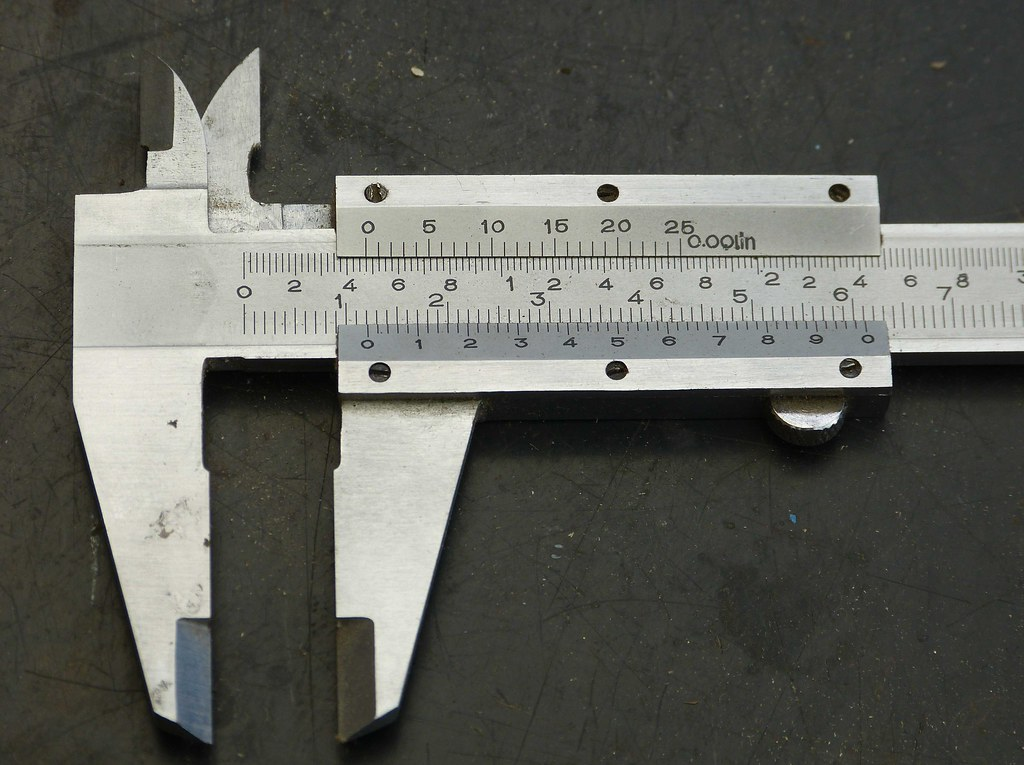
\includegraphics[width=\marginparwidth]{instruments-caliper}\\Margin notes may contain figures, too.} is a section whose title is rendered in orange. For your convenience, you may want to change the name and the color of a section. This can be done in the {\tt gobook.cls} file. 

All sections occupy only part of the page, the rest being used for margin notes. Note that you can include figures in margin notes, too. 
\lipsum[5]

Bibliography\index{bibliography} follows usual rules~\cite{Popper, 1959}\index{Popper, Karl}. \lipsum[6].

Anectods are full width boxes (the width must be manually adjusted as below).
\begin{adjmulticols}{1}{0pt}{-\marginparwidth}
\begin{anecdote}[frametitle=The evolution of cosmology]\index{cosmology}
\lipsum[7-8]
\end{anecdote}
\end{adjmulticols}
Equations can be rendered using {\tt \textbackslash{beq}} and~{\tt \textbackslash{eeq}}:
\beq\label{eq:a.eq.f.over.m}
a=\frac{F}{m}\,.
\eeq
\lipsum[9-10]

\hardware{This is hardware}
\lipsum[12-13]

\more{This is more}
\lipsum[14-15]

\chapter*{Summary}
\begin{adjmulticols}{2}{0pt}{-\marginparwidth}
At the end of a chapter I usually insert a summary full width section. Not mandatory, of course.

\lipsum[11]
\end{adjmulticols}

\begin{thebibliography}{99}
\bibitem{Popper, 1959}Popper, Karl R. The Logic of Scientific Discovery. London: Hutchinson, 1959.
\end{thebibliography}
